\documentclass[12pt,a4paper]{article}
\usepackage[utf8]{inputenc}
\usepackage[german]{babel}
\usepackage[T1]{fontenc}
\usepackage{amsmath}
\usepackage{amsfonts}
\usepackage{amssymb}
\usepackage{graphicx}
\usepackage[left=3cm,right=3cm,top=3cm,bottom=3cm]{geometry}
\usepackage[table]{xcolor}
\usepackage{hyperref}
\setlength{\parskip}{3mm}
\setlength{\parindent}{0cm}
\DeclareMathOperator\erf{erf}
\author{Maike Meier and Lasse Schuirmann}
\title{Messtechnik und Messdatenverarbeitung - Blatt 7}
\newcommand*{\blankpage}{
  \vspace*{\fill}
  \begin{flushright}
  \tiny THIS PAGE INTENTIONALLY LEFT BLANK.
  \end{flushright}
  \pagebreak
}
\begin{document}
\rowcolors{2}{gray!25}{white}

\maketitle
\pagebreak

\blankpage

\section*{Aufgabe 1}
\subsection*{1.1. Welcher Test}
Um eine Ablösung des Sensors zu detektieren, kann der $\chi^2$-Verteilung Anpassungstest durchgeführt werden. (Die Normalverteilung lässt sich ab ca. $n=30$ durch eine $\chi^2$-Verteilung approximieren.)

Eine Voraussetzung für diesen Test ist, dass die Messwerte statistisch unabhängig sind und eine große Stichprobe vorhanden ist.

Der Test kann wie folgt durchgeführt werden:

\begin{enumerate}
\item Voraussetzungen sicherstellen
\item Klassen festlegen, Häufigkeiten $n_i$ bestimmen
\item Null- und Alternativhypothese aufstellen:
\begin{itemize}
 \item[$H_0$] Die Daten sind normalverteilt
 \item[$H_1$] Die Daten sind nicht normalverteilt
\end{itemize}
\item Signifikanzniveau wählen
\item $\chi^2 \approx \sum\limits_{i=1}^8 \frac{(n_i -n p_i)^2}{n p_i}$ berechnen
\item Nullhypothese annehmen oder ablehnen
\end{enumerate}

\subsection*{1.2. Klasseneinteilung}
\scalebox{0.78}{
 \begin{tabular}{|r|c|c|c|c|c|c|c|c|}
 \hline
 \rowcolor{gray!50}
 Klasse & $\leq 35.0$ & $35.1 - 35.5$ & $35.6 - 36.0$ & $36.1 - 36.5$ & $36.6 - 37.0$ & $37.1 - 37.5$ & $37.6 - 38.0$ & $\geq 38.0$ \\
 Anzahl $n_i$ & $4$ & $9$ & $16$ & $20$ & $16$ & $16$ & $6$ & $8$ \\
 \hline
 \end{tabular}}

\noindent
\begin{minipage}{0.6\textwidth}
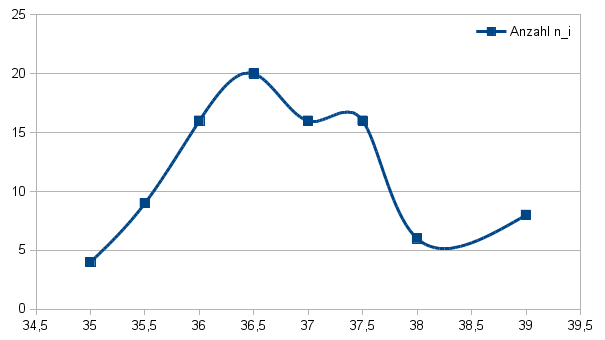
\includegraphics[scale=0.56]{1_2_diagram}
Diagramm 1.
\\
\end{minipage}
\begin{minipage}{0.4\textwidth}
Das Nebenstehende Diagramm ist eine Visualisierung der Obenstehenden Tabelle. (Hierbei wurde ein Datenpunkt jeweils bei einer Oberen Grenze der Klasse gezeichnet.)

Da jede Klasse nicht zu wenige Elemente enthält, das Diagramm aber aussagekräftig scheint, ist diese Einteilung bei dieser Stichprobenmenge sinnvoll.
\end{minipage}

\subsection*{1.3. Erwartete Häufigkeiten}
Die $p_i$s können mithilfe der gegebenen Daten aus einer Normalverteilung errechnet werden. Die gegebene Normalverteilungsfunktion ist im folgenden Diagramm dargestellt:

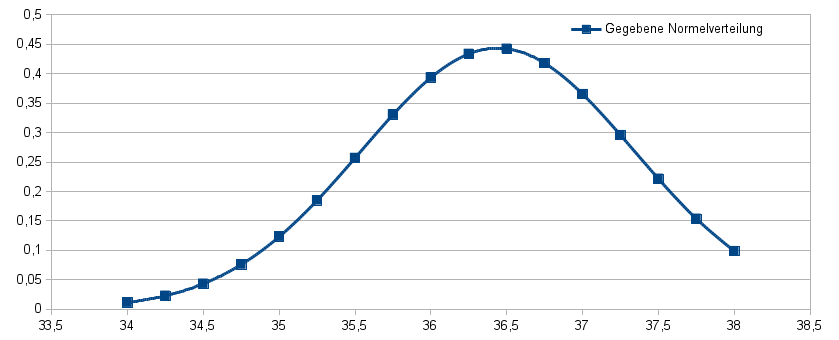
\includegraphics[scale=0.7]{1_3_normvert}

Ermittelt man die Werte der Dichtefunktion zu den gegebenen Klassengrenzen (mit $n$ multipliziert) erhält man folgendes Diagramm:

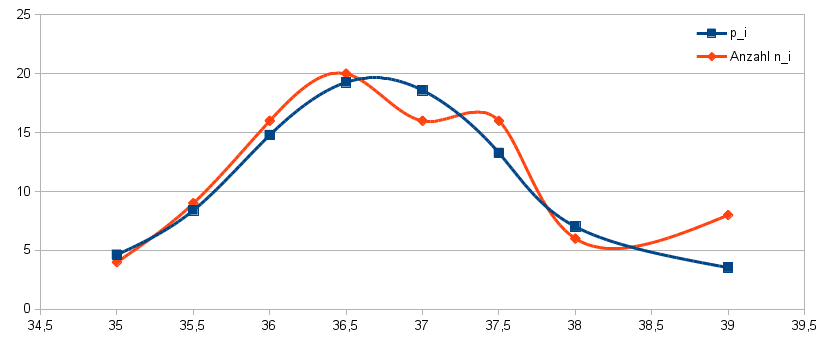
\includegraphics[scale=0.7]{1_3_dichte_vs_data}

\tiny (Alle Datenpunkte bis auf der letzte des Graphen für $n p_i$ stellen wieder die obere Grenze für die Klasse dar. Der Ausnahmepunkt ist der Klasse $38 - \infty$ zuzuordnen, die in unserer Stichprobe keine Werte $> 39$ enthält.)\normalsize

Die dazugehörige Tabelle ist (Werte abgerundet [Informatiker] auf die erste Stelle nach dem Komma):

\scalebox{0.78}{
 \begin{tabular}{|r|c|c|c|c|c|c|c|c|}
 \hline
 \rowcolor{gray!50}
 Klasse & $\leq 35.0$ & $35.1 - 35.5$ & $35.6 - 36.0$ & $36.1 - 36.5$ & $36.6 - 37.0$ & $37.1 - 37.5$ & $37.6 - 38.0$ & $\geq 38.0$ \\
 Anzahl $n_i$ & $4$ & $9$ & $16$ & $20$ & $16$ & $16$ & $6$ & $8$ \\
 $p_i$ & $4.6$ & $8.4$ & $14.7$ & $19.2$ & $18.5$ & $13.2$ & $7.0$ & $3.5$ \\
 \hline
 \end{tabular}}
\subsection*{1.4. Prüfgröße und Vertrauensniveau}
\[
\chi^2 \approx \sum\limits_{i=1}^8 \frac{(n_i -n p_i)^2}{n p_i} \approx 6,27 (= 0,18+0,04+0,1+0,02+0,36+0,56+0,15+4,86)
\]

Also mit $\mu \approx 36.44$:

\[
P(6.28) = \int\limits_{30.16}^{42.72} \mathcal{N}(x) dx \approx 1
\]

\tiny Die Differenz des realen Ergebnis' zu $1$ ist außerhalb der double Rechnergenauigkeit.\normalsize

Damit gilt $P > 1-\alpha$ für übliche $\alpha$ und die Nullhypothese wird abgelehnt.

\subsection*{1.5. Interpretation}
Die Ergebnisse, wie auch Anfangs die Diagramme, legen klar dar, dass es sich nicht um eine Normalverteilte Größe handelt. Es ist also sehr Wahrscheinlich, dass sich der Sensor von dem Probanden gelöst hat.

\pagebreak
\section*{Aufgabe 2}
\subsection*{2.1. Toleranzgrenzen}
Toleranzgrenzen sind die Grenzen in denen ungefähr $99.73\%$ ($\mu \pm 3\sigma$) aller Messwerte liegen müssen.

\subsection*{2.2. Standardabweichung und Toleranzfeldmittenabweichung}
Die Standardabweichung der gegebenen Daten ist $\sigma \approx 0.1$.

Die Abweichung des Mittelwerts $\hat{x}$ von der Toleranzfeldmitte ist $\Delta \hat{x} \approx 3.3$.

\subsection*{2.3. Visualisierung}

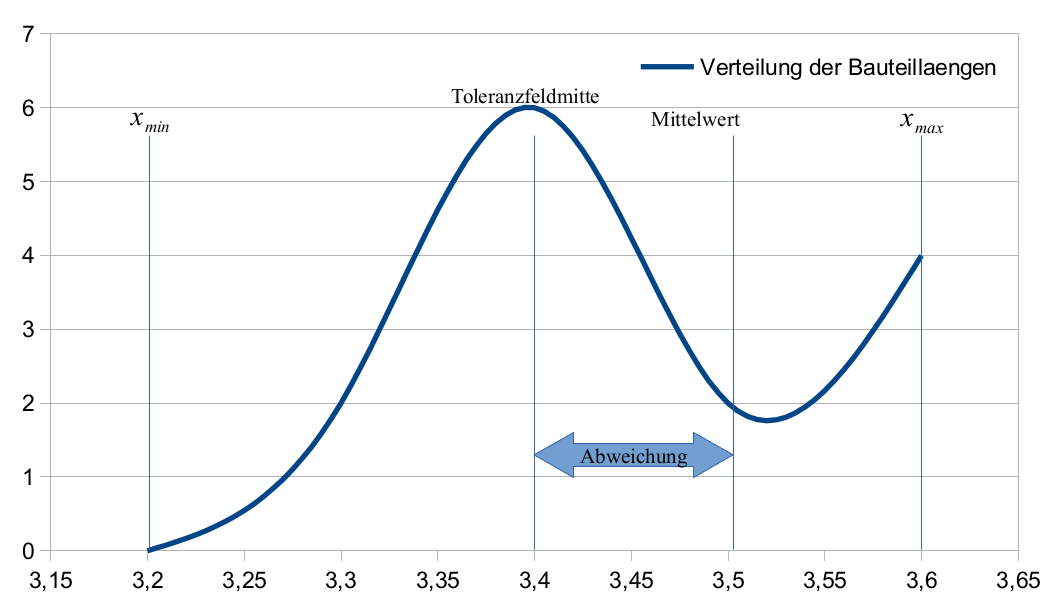
\includegraphics[scale=0.40]{2_3_diag}

\subsection*{2.4. Prozessfähigkeitsindex}

Der Prozessfähigkeitsindex ist $c_p = \frac{x_{max} - x_{min}}{6\sigma} \approx 0.63$.

Wenn $c_p \geq 1$ und $c_{pk} \geq 1$ gibt es weniger als $0.27\%$ Ausschuss.

\subsection*{2.5. Prozessbrauchbarkeitsindex}
Der Prozessbrauchbarkeitsindex ist $c_{pk} = c_p \left(1-\frac{\Delta \hat{x}}{\Delta x_s}\right) \approx 0.47$.

\subsection*{2.6. Ausschuss}
Der Ausschuss beträgt:

\[
p \approx \frac{1 - \erf\left(\frac{3 c_{pk}}{\sqrt{2}}\right)}{2} \approx 0.08
\]

\pagebreak
\section*{Aufgabe 3}
\subsection*{3.1. Genauigkeitsklasse}
Die Genauigkeit $G = \left| \frac{\Delta x_{max}}{u_e} \right|$ ist der maximale Fehler relativ zu dem gegebenen Messbereich. Dieser Wert ist für beide Geräte mit $4\%$ und $7\%$ gegeben. Da also für beide Geräte $G < 0.1$ gilt, fallen beide in die Kategorie der Feinmessgeräte.

\subsection*{3.2. Varianz}
Stellt man den gegebenen Zusammenhang um, erhält man:

\[
\frac{U \cdot F}{R \cdot T} = \ln(pH - 7) \Rightarrow \exp\left(\frac{U \cdot F}{R \cdot T}\right) = pH - 7
\]

Also:

\[
\frac{(1 + \Delta U) \cdot U \cdot F}{(1 + \Delta T) \cdot T \cdot R} = \ln(pH - 7) \Rightarrow \exp\left(\frac{(1 + \Delta U) \cdot U \cdot F}{(1 + \Delta T) \cdot T \cdot R}\right) = pH - 7
\]

Mit $Var(U) = \sigma_U^2$ ergibt sich für die Varianz $1 + \Delta U = 1.0001$ und $1 + \Delta T = 1.02$. Dann ist der Fehler des Terms $\frac{U \cdot F}{R \cdot T}$ durch $\frac{(1 + \Delta U) \cdot U \cdot F}{(1 + \Delta T) \cdot T \cdot R} \approx 0.98 \cdot \frac{U \cdot F}{T \cdot R}$ bestimmt, also ein Fehler von ungefähr $2\%$.

Es gelte nun $g = \frac{U \cdot F}{R \cdot T}$. Also $\exp(g) = pH - 7$ und $\Delta g = 0.02$. Nun ist der relative Fehler für $\exp(g)$ gegeben durch $\Delta pH = exp(g) \cdot (1 + \Delta g) - 1 = exp\left(\frac{U \cdot F}{R \cdot T}\right) \cdot 1.02 -1$.
\begin{flushright}
$\square$
\end{flushright}

\subsection*{3.3. Maximaler Relativer Fehler}
TODO Fehlerfortpflanzung...

\end{document}